%!TeX root=../tese.tex
%("dica" para o editor de texto: este arquivo é parte de um documento maior)
% para saber mais: https://tex.stackexchange.com/q/78101/183146

% Vamos definir alguns comandos auxiliares para facilitar.

% "textbackslash" é muito comprido.
\newcommand{\sla}{\textbackslash}

% Vamos escrever comandos (como "make" ou "itemize") com formatação especial.
\newcommand{\cmd}[1]{\textsf{#1}}

% Idem para packages; aqui estamos usando a mesma formatação de \cmd,
% mas poderíamos escolher outra.
\newcommand{\pkg}[1]{\textsf{#1}}

% A maioria dos comandos LaTeX começa com "\"; vamos criar um
% comando que já coloca essa barra e formata com "\cmd".
\newcommand{\ltxcmd}[1]{\cmd{\sla{}#1}}

\chapter{O Problema do Ancestral de Nível e Implementações}
\label{chap:implementacoes}

\section{Definição do problema}
O problema do \textbf{Ancestral de Nível} é um problema fundamental de árvores que pode
ser definido da seguinte forma: Dada uma árvore enraizada $T$ com $n$ nós, para
consultas $\mathrm{AN}(u, d)$ onde $u$ é um nó de $T$ e $d$ um número inteiro,
encontre o ancestral de profundidade $d$ de $u$ otimizando tanto o tempo de
preprocessamento quanto o de resposta às consultas.

\tikzset{
  treenode/.style = {align=center, minimum size=7mm, inner sep=0pt, text centered},
  arn_n/.style = {treenode, circle, white, font=\bfseries, draw=black,
    fill=black, text width=1.5em},% arbre rouge noir, noeud noir
  arn_r/.style = {treenode, circle, red, draw=red, 
    text width=1.5em, very thick},% arbre rouge noir, noeud rouge
  arn_x/.style = {treenode, circle, draw=black, minimum size=7mm}% arbre rouge noir, nil
}

\begin{figure}[H]
    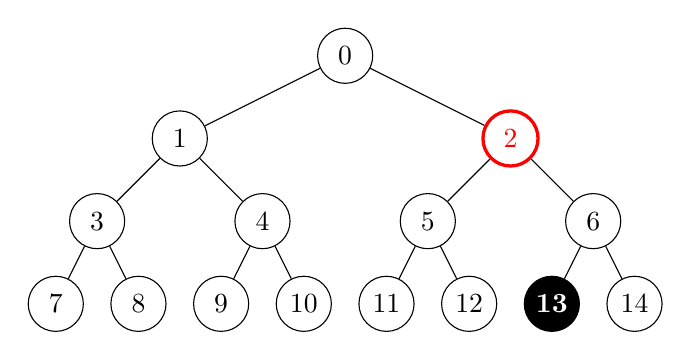
\begin{tikzpicture}[scale=0.7,
      level distance=1.5cm,
      level 1/.style={sibling distance=6cm},
      level 2/.style={sibling distance=3cm},
      level 3/.style={sibling distance=1.5cm}]
      \node [arn_x] {0}
        child {node [arn_x] {1}
          child {node [arn_x] {3}
            child {node [arn_x] {7}}
            child {node [arn_x] {8}}
          }
          child {node [arn_x] {4}
            child {node [arn_x] {9}}
            child {node [arn_x] {10}}
          }
        }
        child {node [arn_r] {2}
          child {node [arn_x] {5}
            child {node [arn_x] {11}}
            child {node [arn_x] {12}}
          }
          child {node [arn_x] {6}
              child {node [arn_n] {13}}
              child {node [arn_x] {14}}
          }
        };
    \end{tikzpicture}
    \caption[Exemplo de consulta de Ancestral de Nível]
    {Exemplo de consulta AN(13, 1) = 2.}
  \end{figure}

  \begin{figure}[H]
    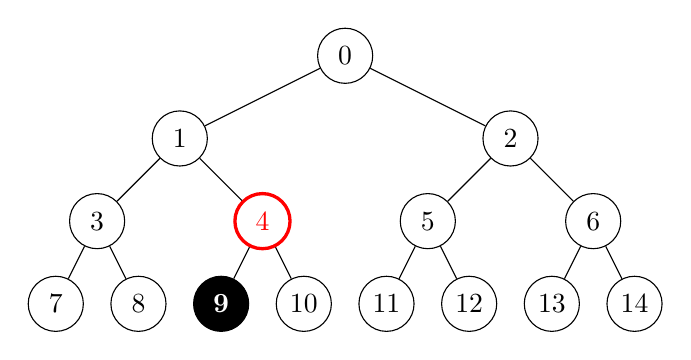
\begin{tikzpicture}[scale=0.7,
        level distance=1.5cm,
        level 1/.style={sibling distance=6cm},
        level 2/.style={sibling distance=3cm},
        level 3/.style={sibling distance=1.5cm}]
        \node [arn_x] {0}
          child {node [arn_x] {1}
            child {node [arn_x] {3}
              child {node [arn_x] {7}}
              child {node [arn_x] {8}}
            }
            child {node [arn_r] {4}
              child {node [arn_n] {9}}
              child {node [arn_x] {10}}
            }
          }
          child {node [arn_x] {2}
            child {node [arn_x] {5}
              child {node [arn_x] {11}}
              child {node [arn_x] {12}}
            }
            child {node [arn_x] {6}
                child {node [arn_x] {13}}
                child {node [arn_x] {14}}
            }
          };
      \end{tikzpicture}
      \caption[Exemplo de consulta de Ancestral de Nível]
      {Exemplo de consulta AN(9, 2) = 4.}
    \end{figure}

Existem diversas soluções para tal problema, de diferentes níveis de complexidade e
com performances teoricamente diferentes. Em particular, por exemplo, é possível
realizar as consultas de forma trivial sem qualquer tipo de preprocessamento ou também
preprocessar todas as possíveis consultas para que possam então ser respondidas
rapidamente.

Em \citet{Bender2002TheLA}, \citet{LAInPractice} e \citet{menghani2019simple} são
discutidas algumas soluções, incluindo as que serão implementadas e testadas neste
trabalho. Em particular, preferi testar soluções que fossem razoavelmente simples
de serem implementadas, até mesmo para mostrar que estas são muitas vezes bastante
suficientes.

Como motivação para o estudo deste problema, vale lembrar que o Ancestral de Nível
aparece como parte de problemas mais complexos como árvores ordinais espaço-eficientes
como descrito em \citet{Geary:2006:SOT:1198513.1198516} que podem ser usadas na
representação de documentos XML que suportam consultas XPath. Além disso, são usadas
em \citet{Sadakane:2006:SSD:1109557.1109693} para implementar estruturas de dados
comprimidas e também em \citet{Yuan:2009:EDS:1514894.1514908} para consultas agregadas
em árvores. Por último, vemos aplicações até mesmo no campo de \textit{hashing} em
strings, como dito em \citet{10.1007/3-540-61258-0_11}.

\section{Implementações}

Todas as implementações assumem a mesma implementação de árvore onde é
guardada apenas sua raíz e cada nó contém um vetor de ponteiros para seus
filhos. Para facilitar as implementações, ao construir a árvore é feita uma
busca em profundidade para preencher vetores que servirão como funções globais
\texttt{pai()} e \texttt{profundidade()}.

\begin{program}[H]
  \lstinputlisting[
    language=pseudocode,
    style=pseudocode,
    style=wider,
    functions={travessia},
    specialidentifiers={global},
  ]
  {conteudo-exemplo/tree.psc}

  \caption{Criação da árvore.\label{prog:tree}}
\end{program}

Estamos interessados em analisar, para cada algoritmo, tanto sua complexidade de
tempo de execução quanto a de espaço adicional, também levando em consideração quão
simples é sua implementação.

Para tornar a discussão da complexidade de tempo mais clara, vamos dizer que se um
algoritmo tem complexidade de tempo $\langle f(x), g(x) \rangle$, a complexidade de
seu preprocessamento é $f(x)$ e de suas consultas é $g(x)$.

\subsection{Algoritmo Trivial}

O primeiro algoritmo a ser estudado é um em que simplesmente não há
nenhum preprocessamento e, para cada consulta, apenas subimos pelos pais a
partir do nó em questão até encontrarmos seu ancestral com profundidade igual
à profundidade requisitada.

%\subsection*{Preprocessamento}
Para esta implementação, o tempo de execução de seu preprocessamento não depende do
tamanho da árvore e também não utiliza nenhuma memória adicional, portanto o
preprocessamento do Algoritmo Trivial tem complexidade $\bigO(1)$ tanto para tempo
quanto espaço.

%\subsection*{Consultas}

No que diz respeito a cada consulta, precisamos chamar a função $pai()$
partindo do nó inicial até chegar no nó com a profundidade desejada.
Essa quantidade é exatamente a diferença entre esta profundidade e a
profundidade do nó inicial.

\begin{program}[]
  \lstinputlisting[
    language=pseudocode,
    style=pseudocode,
    style=wider,
    functions={pai, profundidade},
    specialidentifiers={},
  ]
  {conteudo-exemplo/naive_query.psc}

  \caption{Consulta do Algoritmo Trivial.\label{prog:naivequery}}
\end{program}

A consulta mais lenta para uma árvore qualquer é uma que parte do nó mais profundo
e precisa subir até a raíz, levando tempo $\bigO(d)$, onde $d$ é a profundidade
da árvore. No pior caso isso é equivalente a $\bigO(n)$ onde $n$ é a quantidade
de nós e para uma árvore balanceada cujos nós tem $k$ filhos, é equivalente a
$\bigO(\log_k n)$, fazendo com que a performance da consulta seja muito dependente da
forma da árvore.

Após essa análise, podemos concluir que o Algoritmo Trivial tem complexidade de tempo
$\langle \bigO(1), \bigO(d) \rangle$ e $\bigO(1)$ de espaço adicional, sendo
particularmente eficiente para árvores balanceadas e com fator de ramificação maior.


\subsection{Algoritmo da Tabela}
Ao contrário do algoritmo trivial, a ideia é precalcular o resultado de todas
as consultas possíveis durante a fase de preprocessamento para otimizar o
desempenho da fase de consultas.

Cada nó $u$ tem associado a si $profundidade(u) + 1$ possíveis consultas. Assim, para uma
árvore com $n$ nós, existem $n + \sum_{i=0}^{n-1} profundidade(i) = \bigO(nd)$ consultas, onde $d$ é a profundidade da árvore.
O preprocessamento se dá de maneira simples, preenchendo uma tabela de tamanho
$\bigO(nd)$ com dois laços encadeados, utilizando a função $pai()$ para subir a partir
de cada nó até a raíz e salvar a resposta para cada profundidade.

\begin{program}[]
  \lstinputlisting[
    language=pseudocode,
    style=pseudocode,
    style=wider,
    functions={pai, profundidade},
    specialidentifiers={},
  ]
  {conteudo-exemplo/table_preprocessing.psc}

  \caption{Preprocessamento do Algoritmo da Tabela.\label{prog:tableproc}}
\end{program}

Com a tabela devidamente preenchida, as consultas se tornam tão simples quanto acessar
a sua entrada correspondente, ou seja, a resposta da consulta que pede pelo ancestral
do nó $u$ com profundidade $p$ é dada por $tabela[u][p]$. 

\begin{program}[h!]
  \lstinputlisting[
    language=pseudocode,
    style=pseudocode,
    style=wider,
    functions={pai, profundidade},
    specialidentifiers={},
  ]
  {conteudo-exemplo/table_query.psc}

  \caption{Consulta do Algoritmo da Tabela.\label{prog:tablequery}}
\end{program}

A complexidade de espaço e de tempo do preprocessamento dependem fortemente da forma da
árvore, podendo ser $\bigO(n^2)$ no caso de uma árvore linear e para o caso de uma
árvore $k$-ária balanceada é $\bigO(n \log_k n)$, muito mais eficiente. Já a consulta
é feita em tempo $\bigO(1)$, sem uso de espaço adicional. Assim, o Algoritmo da Tabela
tem complexidade de tempo $\langle \bigO(nd), \bigO(1) \rangle$ e $\bigO(nd)$ de espaço,
sendo uma boa opção para casos de árvores balanceadas em que o preprocessamento se torna
barato frente à quantidade de consultas que serão feitas e o espaço utilizado não é
uma restrição.


\subsection{Algoritmo dos Ponteiros}
Essa é possivelmente a solução mais complexa que vamos analisar

\begin{program}[h!]
  \lstinputlisting[
    language=pseudocode,
    style=pseudocode,
    style=wider,
    functions={dfs, filhos, insere},
    specialidentifiers={global},
  ]
  {conteudo-exemplo/jump_preprocess.psc}

  \caption{Preprocessamento do Algoritmo da Preordem.\label{prog:preorderproc}}
\end{program}

\subsection{Algoritmo da Preordem}
O último algoritmo faz uso das propriedades da preordem de uma árvore para trazer uma
solução mais eficiente. Enquanto é feita a travessia da árvore cada nó é associado à
seu índice na preordem, que é inserido numa lista de nós de sua respectiva profundidade.

\begin{figure}
  \centering
  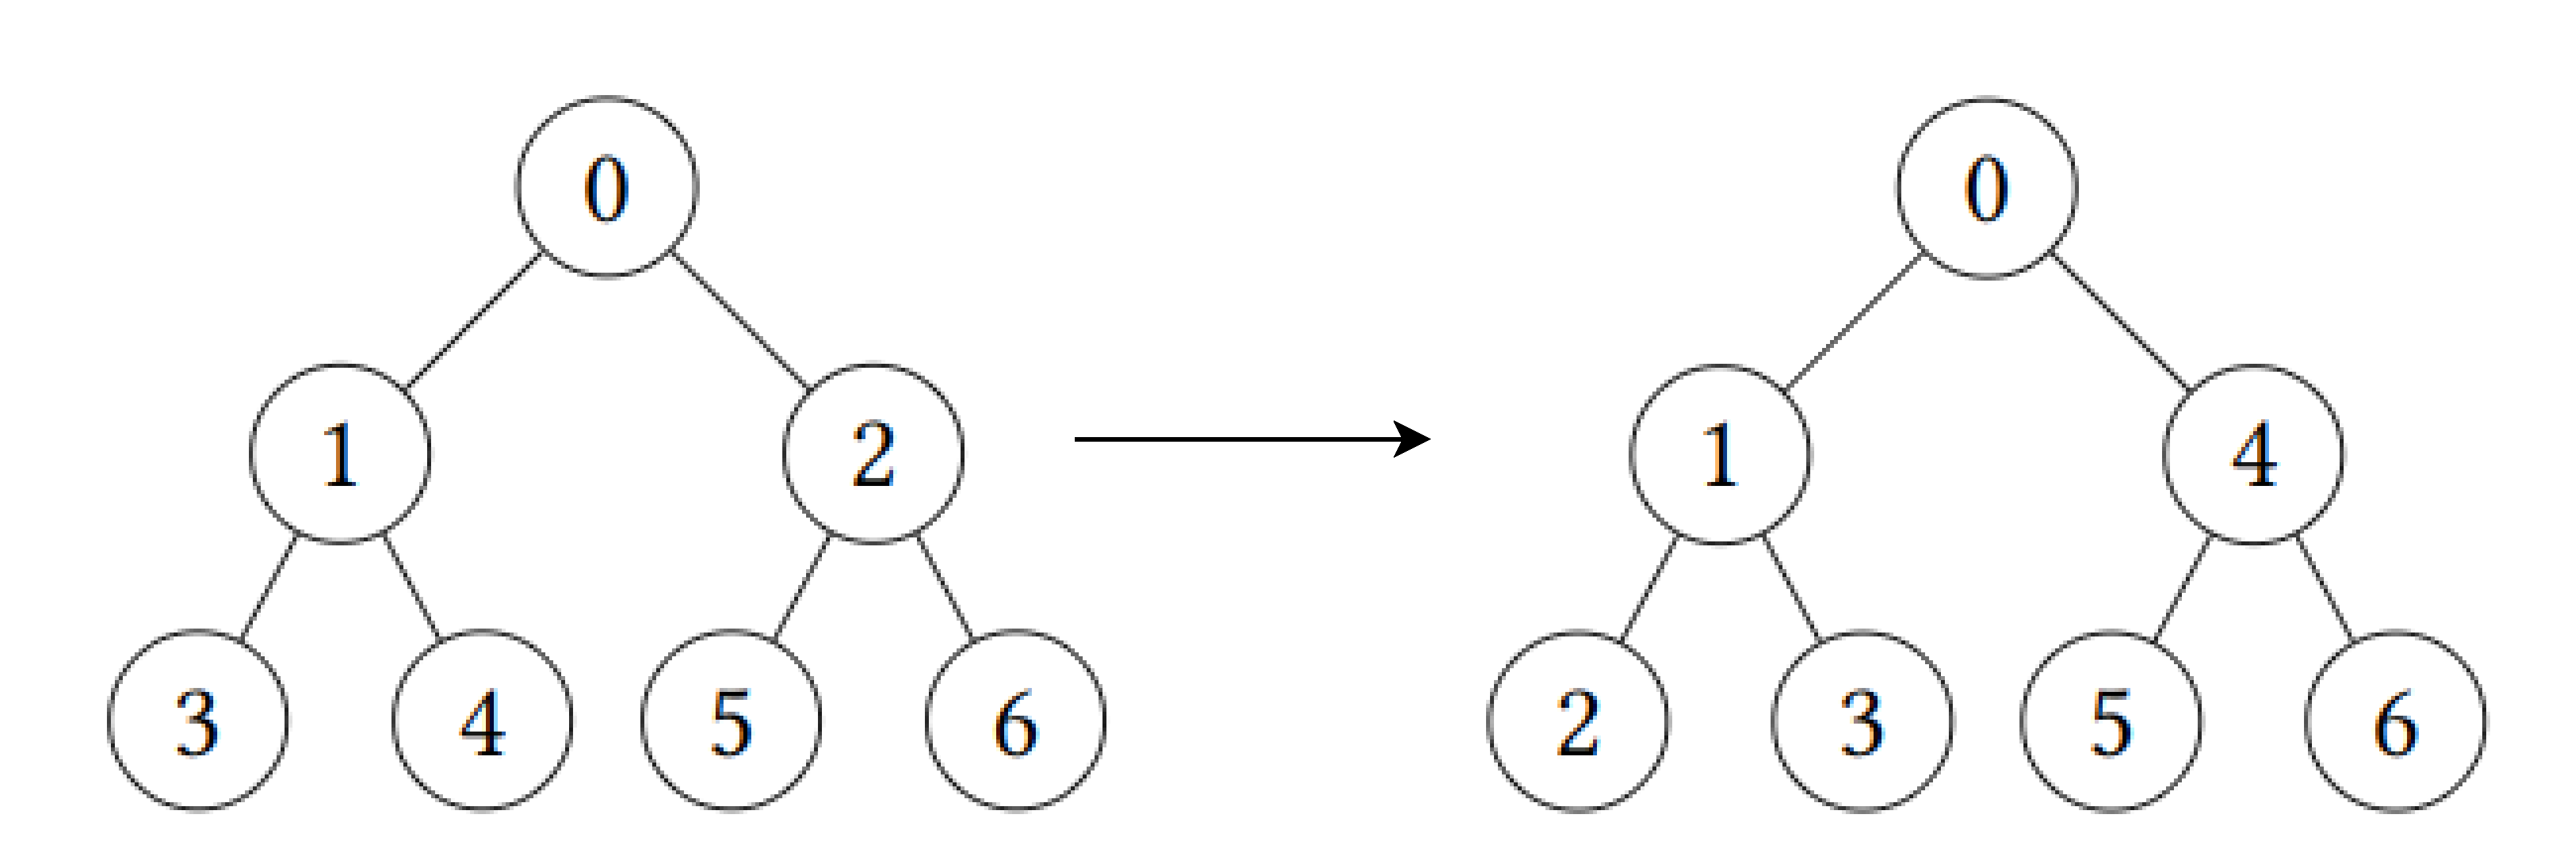
\includegraphics[scale=0.18]{preordertransformation.pdf}
  \caption{Associação entre os índices originais e os índices da preordem.}
\end{figure}

\begin{table}[]
  \begin{tabular}{llllll}
  \cline{3-3}
  profundidade 0: & \multicolumn{1}{l|}{} & \multicolumn{1}{l|}{0} &                        &                        &                        \\ \cline{3-3}
                  &                       &                        &                        &                        &                        \\ \cline{3-4}
  profundidade 1: & \multicolumn{1}{l|}{} & \multicolumn{1}{l|}{1} & \multicolumn{1}{l|}{4} &                        &                        \\ \cline{3-4}
                  &                       &                        &                        &                        &                        \\ \cline{3-6} 
  profundidade 2: & \multicolumn{1}{l|}{} & \multicolumn{1}{l|}{2} & \multicolumn{1}{l|}{3} & \multicolumn{1}{l|}{5} & \multicolumn{1}{l|}{6} \\ \cline{3-6} 
  \end{tabular}
  \caption[Vetores contendo os nós processados em cada nível.]
  {Vetores contendo os nós processados em cada nível. Os índices são referentes à preordem.}
\end{table}

Para tal, a ideia é guardar a ordem em que os nós de cada nível
foram visitados durante a travessia em preordem em vetores e então uma consulta se
resume a procurar o ancestral do nó inicial que está no vetor correspondente à
profundidade buscada.

\begin{program}[h!]
  \lstinputlisting[
    language=pseudocode,
    style=pseudocode,
    style=wider,
    functions={dfs, filhos, insere},
    specialidentifiers={global},
  ]
  {conteudo-exemplo/preorder_preprocess.psc}

  \caption{Preprocessamento do Algoritmo da Preordem.\label{prog:preorderproc}}
\end{program}

Para entendermos o funcionamento do algoritmo para as consultas, primeiro precisamos
nos convencer de que, se um nó $v$ é ancestral de $u$, então $preordem(v) < preordem(u)$,
onde $preordem(x)$ é o índice associado à posição de $x$ na travessia em preordem, já
que sempre descobrimos os filhos de um nó depois dele próprio. Além disso, no caso em
que existam vários nós em determinada profundidade, o ancestral que buscamos é aquele
cujo índice na preordem é o mais próximo do índice do nó inicial, porém ainda menor
que tal.

\begin{program}[]
  \lstinputlisting[
    language=pseudocode,
    style=pseudocode,
    style=wider,
    functions={upper_bound},
    specialidentifiers={},
  ]
  {conteudo-exemplo/preorder_query.psc}

  \caption{Consulta do Algoritmo da Preordem.\label{prog:preorderquery}}
\end{program}

\section{Considerações gerais}
No próximo capítulo estaremos interessados em avaliar a performance de cada algoritmo
para alguns casos de teste, levando em consideração o preprocessamento necessário,
a realização de consultas e a quantidade de memória utilizada.

Entretanto, analisando as tabelas ~\ref{tab:complexidadetempo},
~\ref{tab:complexidadeespaco} podemos perceber de imediato que restringir a entrada
para árvores balanceadas permite até mesmo que os algoritmos mais simples apresentem
complexidades boas, sendo ótimas opções levando em consideração também a dificuldade
de implementação de cada algoritmo.

\begin{table}[]
  \begin{tabular}{|c|l|l|l|}
  \hline
            & Linear                                       & Binária                                      & k-ária                                       \\ \hline
  Trivial   & $\langle \bigO(1), \bigO(n) \rangle$                 & $\langle \bigO(1), \bigO(\log_2 n) \rangle$          & $\langle \bigO(1), \bigO(\log_k n) \rangle$          \\ \hline
  Tabela    & $\langle \bigO(n^2), \bigO(1) \rangle$               & $\langle \bigO(n \log_2 n), \bigO(1) \rangle$        & $\langle \bigO(n \log_k n), \bigO(1) \rangle$        \\ \hline
  Ponteiros & $\langle \bigO(n \log_2 n), \bigO(\log_2 n) \rangle$ & $\langle \bigO(n \log_2 n), \bigO(\log_2 n) \rangle$ & $\langle \bigO(n \log_2 n), \bigO(\log_2 n) \rangle$ \\ \hline
  Preordem  & $\langle \bigO(n), \bigO(1) \rangle$                 & $\langle \bigO(n), \bigO(\log_2 n) \rangle$          & $\langle \bigO(n), \bigO(\log_2 n) \rangle$          \\ \hline
  \end{tabular}
  \caption{Comparação da complexidade de tempo dos algoritmos.\label{tab:complexidadetempo}}
  \end{table}

  \begin{table}[]
    \begin{tabular}{|c|l|l|l|}
    \hline
              & Linear              & Binária             & k-ária              \\ \hline
    Trivial   & $\bigO(1)$          & $\bigO(1)$              & $\bigO(1)$              \\ \hline
    Tabela    & $\bigO(n^2)$        & $\bigO(n \log_2 n)$     & $\bigO(n \log_k n)$ \\ \hline
    Ponteiros & $\bigO(n \log_2 n)$ & $\bigO(n \log_2 n)$ & $\bigO(n \log_2 n)$ \\ \hline
    Preordem  & $\bigO(n)$          & $\bigO(n)$          & $\bigO(n)$          \\ \hline
    \end{tabular}
    \caption{Comparação da complexidade de espaço dos algoritmos.\label{tab:complexidadeespaco}}
    \end{table}
